\documentclass[12pt]{article}
\usepackage{amsmath}
\usepackage{graphicx}

\title{\LaTeX{} Tutorial}
\author{Created by Jeremy Wang}
\date{\today}
\begin{document}
  \maketitle
  \LaTeX{} is a compiler for the \TeX{} typesetting program
  It offers programmable desktop publishing features and extensive facilities for
  automating most aspects of typesetting and desktop
  publishing, including numbering and cross-referencing,
  tables and figures, page layout, bibliographies, and
  much more.
 
  % This is a comment, not shown in final output.
  % The following shows typesetting power of LaTeX:

  \begin{align}
    E_0 &= mc^2                              \\
    E &= \frac{mc^2}{\sqrt{1-\frac{v^2}{c^2}}}
  \end{align}


  \LaTeX{} images!

  \begin{center}
  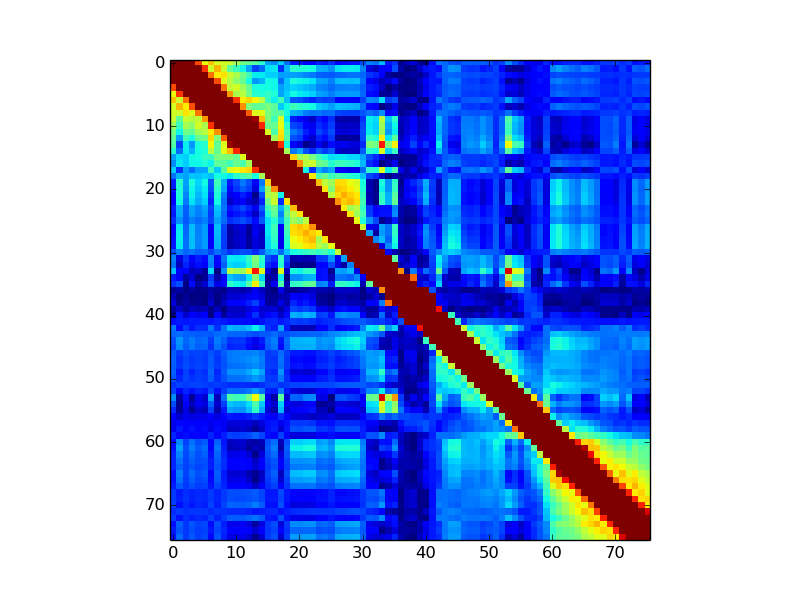
\includegraphics[height=5cm, keepaspectratio]{images/fancy_figure.png}
  \end{center}

\end{document}
